\documentclass[tikz,border=2pt]{standalone}
\usepackage{amsmath,amssymb}
\usepackage{tikz}
\usetikzlibrary{arrows.meta}

\begin{document}
% The Giapetto model: soldiers x_s and trains x_t, profit 3 and 2, finishing hours
% 2 x_s + x_t <= 100, carpentry hours x_s + x_t <= 80, soldier demand x_s <= 40.
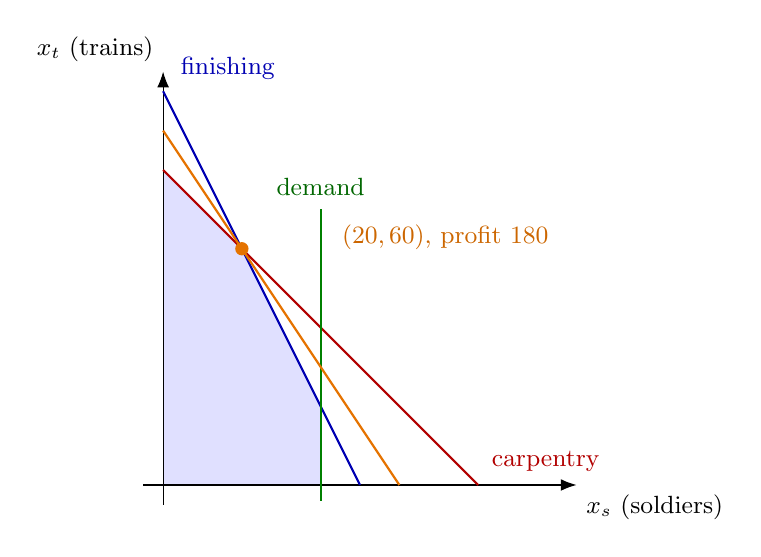
\begin{tikzpicture}[x=0.05cm, y=0.05cm, every node/.style={font=\small}, >={Latex[length=2mm]}]
	\fill[blue!12] (0,0) -- (40,0) -- (40,20) -- (20,60) -- (0,80) -- cycle;
	\draw[->] (-5,0) -- (105,0) node[below right] {$x_s$ (soldiers)};
	\draw[->] (0,-5) -- (0,105) node[above left] {$x_t$ (trains)};
	\draw[blue!70!black, thick] (50,0) -- (0,100);
	\draw[red!70!black, thick] (80,0) -- (0,80);
	\draw[green!50!black, thick] (40,-4) -- (40,70);
	\node[blue!70!black, anchor=south west] at (2,100.5) {finishing};
	\node[red!70!black, anchor=south west] at (81,1) {carpentry};
	\node[green!40!black, anchor=south] at (40,71) {demand};
	\draw[orange!90!black, thick] (60,0) -- (0,90);
	\fill[orange!90!black] (20,60) circle (2.4pt);
	\node[orange!80!black, anchor=west] at (43,63) {$(20,60)$, profit $180$};
	\end{tikzpicture}
\end{document}
